% Options for packages loaded elsewhere
\PassOptionsToPackage{unicode}{hyperref}
\PassOptionsToPackage{hyphens}{url}
\PassOptionsToPackage{dvipsnames,svgnames,x11names}{xcolor}
%
\documentclass[
  letterpaper,
  DIV=11,
  numbers=noendperiod]{scrartcl}

\usepackage{amsmath,amssymb}
\usepackage{iftex}
\ifPDFTeX
  \usepackage[T1]{fontenc}
  \usepackage[utf8]{inputenc}
  \usepackage{textcomp} % provide euro and other symbols
\else % if luatex or xetex
  \usepackage{unicode-math}
  \defaultfontfeatures{Scale=MatchLowercase}
  \defaultfontfeatures[\rmfamily]{Ligatures=TeX,Scale=1}
\fi
\usepackage{lmodern}
\ifPDFTeX\else  
    % xetex/luatex font selection
\fi
% Use upquote if available, for straight quotes in verbatim environments
\IfFileExists{upquote.sty}{\usepackage{upquote}}{}
\IfFileExists{microtype.sty}{% use microtype if available
  \usepackage[]{microtype}
  \UseMicrotypeSet[protrusion]{basicmath} % disable protrusion for tt fonts
}{}
\makeatletter
\@ifundefined{KOMAClassName}{% if non-KOMA class
  \IfFileExists{parskip.sty}{%
    \usepackage{parskip}
  }{% else
    \setlength{\parindent}{0pt}
    \setlength{\parskip}{6pt plus 2pt minus 1pt}}
}{% if KOMA class
  \KOMAoptions{parskip=half}}
\makeatother
\usepackage{xcolor}
\setlength{\emergencystretch}{3em} % prevent overfull lines
\setcounter{secnumdepth}{-\maxdimen} % remove section numbering
% Make \paragraph and \subparagraph free-standing
\ifx\paragraph\undefined\else
  \let\oldparagraph\paragraph
  \renewcommand{\paragraph}[1]{\oldparagraph{#1}\mbox{}}
\fi
\ifx\subparagraph\undefined\else
  \let\oldsubparagraph\subparagraph
  \renewcommand{\subparagraph}[1]{\oldsubparagraph{#1}\mbox{}}
\fi

\usepackage{color}
\usepackage{fancyvrb}
\newcommand{\VerbBar}{|}
\newcommand{\VERB}{\Verb[commandchars=\\\{\}]}
\DefineVerbatimEnvironment{Highlighting}{Verbatim}{commandchars=\\\{\}}
% Add ',fontsize=\small' for more characters per line
\usepackage{framed}
\definecolor{shadecolor}{RGB}{241,243,245}
\newenvironment{Shaded}{\begin{snugshade}}{\end{snugshade}}
\newcommand{\AlertTok}[1]{\textcolor[rgb]{0.68,0.00,0.00}{#1}}
\newcommand{\AnnotationTok}[1]{\textcolor[rgb]{0.37,0.37,0.37}{#1}}
\newcommand{\AttributeTok}[1]{\textcolor[rgb]{0.40,0.45,0.13}{#1}}
\newcommand{\BaseNTok}[1]{\textcolor[rgb]{0.68,0.00,0.00}{#1}}
\newcommand{\BuiltInTok}[1]{\textcolor[rgb]{0.00,0.23,0.31}{#1}}
\newcommand{\CharTok}[1]{\textcolor[rgb]{0.13,0.47,0.30}{#1}}
\newcommand{\CommentTok}[1]{\textcolor[rgb]{0.37,0.37,0.37}{#1}}
\newcommand{\CommentVarTok}[1]{\textcolor[rgb]{0.37,0.37,0.37}{\textit{#1}}}
\newcommand{\ConstantTok}[1]{\textcolor[rgb]{0.56,0.35,0.01}{#1}}
\newcommand{\ControlFlowTok}[1]{\textcolor[rgb]{0.00,0.23,0.31}{#1}}
\newcommand{\DataTypeTok}[1]{\textcolor[rgb]{0.68,0.00,0.00}{#1}}
\newcommand{\DecValTok}[1]{\textcolor[rgb]{0.68,0.00,0.00}{#1}}
\newcommand{\DocumentationTok}[1]{\textcolor[rgb]{0.37,0.37,0.37}{\textit{#1}}}
\newcommand{\ErrorTok}[1]{\textcolor[rgb]{0.68,0.00,0.00}{#1}}
\newcommand{\ExtensionTok}[1]{\textcolor[rgb]{0.00,0.23,0.31}{#1}}
\newcommand{\FloatTok}[1]{\textcolor[rgb]{0.68,0.00,0.00}{#1}}
\newcommand{\FunctionTok}[1]{\textcolor[rgb]{0.28,0.35,0.67}{#1}}
\newcommand{\ImportTok}[1]{\textcolor[rgb]{0.00,0.46,0.62}{#1}}
\newcommand{\InformationTok}[1]{\textcolor[rgb]{0.37,0.37,0.37}{#1}}
\newcommand{\KeywordTok}[1]{\textcolor[rgb]{0.00,0.23,0.31}{#1}}
\newcommand{\NormalTok}[1]{\textcolor[rgb]{0.00,0.23,0.31}{#1}}
\newcommand{\OperatorTok}[1]{\textcolor[rgb]{0.37,0.37,0.37}{#1}}
\newcommand{\OtherTok}[1]{\textcolor[rgb]{0.00,0.23,0.31}{#1}}
\newcommand{\PreprocessorTok}[1]{\textcolor[rgb]{0.68,0.00,0.00}{#1}}
\newcommand{\RegionMarkerTok}[1]{\textcolor[rgb]{0.00,0.23,0.31}{#1}}
\newcommand{\SpecialCharTok}[1]{\textcolor[rgb]{0.37,0.37,0.37}{#1}}
\newcommand{\SpecialStringTok}[1]{\textcolor[rgb]{0.13,0.47,0.30}{#1}}
\newcommand{\StringTok}[1]{\textcolor[rgb]{0.13,0.47,0.30}{#1}}
\newcommand{\VariableTok}[1]{\textcolor[rgb]{0.07,0.07,0.07}{#1}}
\newcommand{\VerbatimStringTok}[1]{\textcolor[rgb]{0.13,0.47,0.30}{#1}}
\newcommand{\WarningTok}[1]{\textcolor[rgb]{0.37,0.37,0.37}{\textit{#1}}}

\providecommand{\tightlist}{%
  \setlength{\itemsep}{0pt}\setlength{\parskip}{0pt}}\usepackage{longtable,booktabs,array}
\usepackage{calc} % for calculating minipage widths
% Correct order of tables after \paragraph or \subparagraph
\usepackage{etoolbox}
\makeatletter
\patchcmd\longtable{\par}{\if@noskipsec\mbox{}\fi\par}{}{}
\makeatother
% Allow footnotes in longtable head/foot
\IfFileExists{footnotehyper.sty}{\usepackage{footnotehyper}}{\usepackage{footnote}}
\makesavenoteenv{longtable}
\usepackage{graphicx}
\makeatletter
\def\maxwidth{\ifdim\Gin@nat@width>\linewidth\linewidth\else\Gin@nat@width\fi}
\def\maxheight{\ifdim\Gin@nat@height>\textheight\textheight\else\Gin@nat@height\fi}
\makeatother
% Scale images if necessary, so that they will not overflow the page
% margins by default, and it is still possible to overwrite the defaults
% using explicit options in \includegraphics[width, height, ...]{}
\setkeys{Gin}{width=\maxwidth,height=\maxheight,keepaspectratio}
% Set default figure placement to htbp
\makeatletter
\def\fps@figure{htbp}
\makeatother

\KOMAoption{captions}{tableheading}
\makeatletter
\makeatother
\makeatletter
\makeatother
\makeatletter
\@ifpackageloaded{caption}{}{\usepackage{caption}}
\AtBeginDocument{%
\ifdefined\contentsname
  \renewcommand*\contentsname{Table of contents}
\else
  \newcommand\contentsname{Table of contents}
\fi
\ifdefined\listfigurename
  \renewcommand*\listfigurename{List of Figures}
\else
  \newcommand\listfigurename{List of Figures}
\fi
\ifdefined\listtablename
  \renewcommand*\listtablename{List of Tables}
\else
  \newcommand\listtablename{List of Tables}
\fi
\ifdefined\figurename
  \renewcommand*\figurename{Figure}
\else
  \newcommand\figurename{Figure}
\fi
\ifdefined\tablename
  \renewcommand*\tablename{Table}
\else
  \newcommand\tablename{Table}
\fi
}
\@ifpackageloaded{float}{}{\usepackage{float}}
\floatstyle{ruled}
\@ifundefined{c@chapter}{\newfloat{codelisting}{h}{lop}}{\newfloat{codelisting}{h}{lop}[chapter]}
\floatname{codelisting}{Listing}
\newcommand*\listoflistings{\listof{codelisting}{List of Listings}}
\makeatother
\makeatletter
\@ifpackageloaded{caption}{}{\usepackage{caption}}
\@ifpackageloaded{subcaption}{}{\usepackage{subcaption}}
\makeatother
\makeatletter
\@ifpackageloaded{tcolorbox}{}{\usepackage[skins,breakable]{tcolorbox}}
\makeatother
\makeatletter
\@ifundefined{shadecolor}{\definecolor{shadecolor}{rgb}{.97, .97, .97}}
\makeatother
\makeatletter
\makeatother
\makeatletter
\makeatother
\ifLuaTeX
  \usepackage{selnolig}  % disable illegal ligatures
\fi
\IfFileExists{bookmark.sty}{\usepackage{bookmark}}{\usepackage{hyperref}}
\IfFileExists{xurl.sty}{\usepackage{xurl}}{} % add URL line breaks if available
\urlstyle{same} % disable monospaced font for URLs
\hypersetup{
  pdftitle={Banco Federal de Finanças Report},
  pdfauthor={Team 4},
  colorlinks=true,
  linkcolor={blue},
  filecolor={Maroon},
  citecolor={Blue},
  urlcolor={Blue},
  pdfcreator={LaTeX via pandoc}}

\title{Banco Federal de Finanças Report}
\usepackage{etoolbox}
\makeatletter
\providecommand{\subtitle}[1]{% add subtitle to \maketitle
  \apptocmd{\@title}{\par {\large #1 \par}}{}{}
}
\makeatother
\subtitle{Target Marketing Campaign}
\author{Team 4}
\date{}

\begin{document}
\maketitle
\ifdefined\Shaded\renewenvironment{Shaded}{\begin{tcolorbox}[interior hidden, enhanced, breakable, frame hidden, borderline west={3pt}{0pt}{shadecolor}, boxrule=0pt, sharp corners]}{\end{tcolorbox}}\fi

\hypertarget{background}{%
\subsection{Background}\label{background}}

\emph{A major telemarketing campaign and the results were inadequete to
come to a conclusion. We were assigned to impelment a Machine Learning
Algorithim to help find the following:}

\emph{1. Find interesting customer segments based on their previous
marketing campaign.} \emph{2. Find a way to identify the types of
customers most likely to respond favorably to future marketing
campaigns.} \emph{3.Proving to a skeptical Senhor Ferreira that a
targeted campaign based on data science will significantly outperform a
campaign made up of randomly selected customers.}

\emph{Since we're operating in the European Union, we're subject to GDPR
compliance requirements. The GDPR doesn't apply in this situation, since
we're just building a model, not selling data. In order to use this data
under GDPR, we'll need to get consent from the customers in the dataset.
We are also using only historic data that has been put into an anonymous
format so we will be compliant in that department as well.}

\hypertarget{recommendation}{%
\subsection{Recommendation}\label{recommendation}}

\emph{.}

\hypertarget{methodology}{%
\subsection{Methodology}\label{methodology}}

\emph{We decided that using a supervised approach would be ideal for
this job because we are trying to classify our clientele would have
interest in subscribing to a term deposit. Supervised approaches are
better for getting a finite answer. When we took our data we decided
that use eighty percent of the data for training and the remaining data
for testing and validation. We chose this distribution due to this being
a relatively small dataset and is the standard distribution for
supervised learning models.}

\emph{Before we even started applying the data to our learning model. We
needed to adjust some of our data to make it more usable. We changed how
recently people had been contacted to move the people who had not been
contacted into separate groups. We also made it a point to put our
numeric data in groups not using them as individuals.}

\hypertarget{results-actions-and-limitations}{%
\subsection{Results, Actions, and
Limitations}\label{results-actions-and-limitations}}

\emph{.}

\hypertarget{tree}{%
\subsection{Tree}\label{tree}}

\emph{For our model, we decided to use the RandomForestClassifier which
constructs multiple decision trees during the training phase and then
combines their predictions to produce more accurate and stable results.
We augmented the RandomForestClassifier using hyperparameters which
controlled certain aspects of the final decision tree, including the
number of trees in the forest, the max depth of each tree, and the
number of samples required to split an internal node. The
hyperparameters are determined by using GridSearchCV, which will search
over a specified parameter grid, and determine the best parameters by
which we should control the decision tree.}

\hypertarget{metrics}{%
\subsection{Metrics}\label{metrics}}

We decided the most important metric is recall. We wanted to make sure
we get as many yes's with the least amount of calls. Then precesion is
the next important. The data we validated our model with included 3,707
pepole. Of those people we predicted that 3,456 would say no and 251
would say yes. We had a 28.7\% recall and a 52.2\% precision. This means
that our model only got around 30\% of the people that said yes. But
over half of the people the model said was a yes, would actually agree
to the campaign. This means that every other person you call will agree
to the campaign. So we weren't able to get all the people that would say
yes, but we cut out over 3,100 calls out. So you would be able to save a
lot of time and money cutting out all the other calls you would have
been making.

\begin{Shaded}
\begin{Highlighting}[]
\NormalTok{disp }\OperatorTok{=}\NormalTok{ ConfusionMatrixDisplay.from\_estimator(}
\NormalTok{  clf,}
\NormalTok{  X\_test,}
\NormalTok{  y\_test,}
\NormalTok{  cmap}\OperatorTok{=}\NormalTok{plt.cm.Blues,)}
\NormalTok{plt.show()}
\end{Highlighting}
\end{Shaded}

\begin{figure}[H]

{\centering 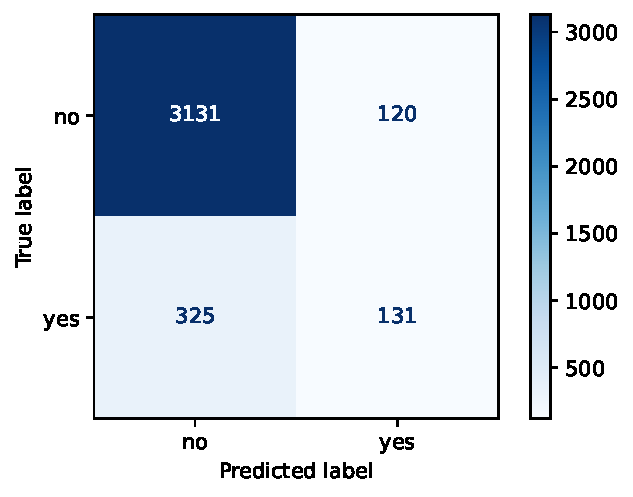
\includegraphics{Executive-summary_files/figure-pdf/cell-4-output-1.pdf}

}

\end{figure}

\hypertarget{questions}{%
\subsection{Questions}\label{questions}}

\textbf{Types of customers respond better on certain days than others?}

\begin{Shaded}
\begin{Highlighting}[]
\CommentTok{\#chart3}
\end{Highlighting}
\end{Shaded}

\emph{We wanted to see which of the two methods of contact would have
the highest success rate from the marketing campaign. As you can see,
Contacting people using a Cellular device would be more benificial than
call those with a telephone. We also can see that Retired and Student
have a 31.59\% and 36.33\% chance of a success rate.}

\begin{Shaded}
\begin{Highlighting}[]
\CommentTok{\#chart2}
\end{Highlighting}
\end{Shaded}

\emph{Looking more into the Student side in which day would be best and
to know if they were Divorced,Married, or Single had help drill in our
target audience. Based on Single section, we can see that during the
middle of the week has a higher chance of gaining a successful call. We
also see that we gain nothing by calling Divorced Students.}

\begin{Shaded}
\begin{Highlighting}[]
\CommentTok{\#chart1}
\end{Highlighting}
\end{Shaded}

\emph{Looking more into the Retired side, we also wanted to know which
marital status would be best to call. The pattern for Retired and
Students seems to be the same where they would be more successfull by
calling in the middle of the week (Tueday through Thrursday) than any
other week.}

\hypertarget{python-notebooks}{%
\subsection{Python Notebooks}\label{python-notebooks}}



\end{document}
